\documentclass[
%% TIKZ_CLASSOPTION %%
tikz
]{standalone}
\usepackage{amsmath}
\usetikzlibrary{matrix}
%% EXTRA_TIKZ_PREAMBLE_CODE %%
\begin{document}
%% TIKZ_CODE %%
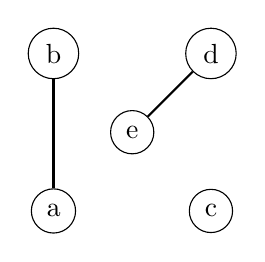
\begin{tikzpicture}

\tikzset{vertex/.style = {shape=circle,draw,minimum size=1.5em}}
\tikzset{edge/.style = {->,> = latex}}

\node[vertex] (a) at (0,0) {a};
\node[vertex] (b) at (0, 2) {b};
\node[vertex] (c) at (2, 0) {c};
\node[vertex] (d) at (2, 2) {d};
\node[vertex] (e) at (1, 1) {e};

\draw[thick] (a) -- (b);
\draw[thick] (d) -- (e);

\end{tikzpicture}
\end{document}
